\subsection{Analiza deskryptywna zmiennych demograficznych}
        \subsubsection*{Wiek}
        \begin{table}[H]
            \centering
            \caption{Opis deskryptywny wieku uczestników badania.}
            \begin{tabular}{|c|c|c|c|}%
                \hline
                \bfseries Miara & \bfseries Gogle przezroczyste & \bfseries Gogle czerwone & \bfseries Gogle żółte% specify table head
                \csvreader[head to column names]{./../res_tables/summaryAge.csv}{}% use head of csv as column names
                {\\\hline\Miara & \num{\T} & \num{\R} & \num{\Y}}% specify your columns here
                \\\hline    
            \end{tabular}
            \label{tab:summaryAge}
        \end{table}

        \begin{figure}[H]
            \centering
            \caption{Histogram dla wieku uczestników badania.}
            \resizebox{0.7 \columnwidth}{!}{%
            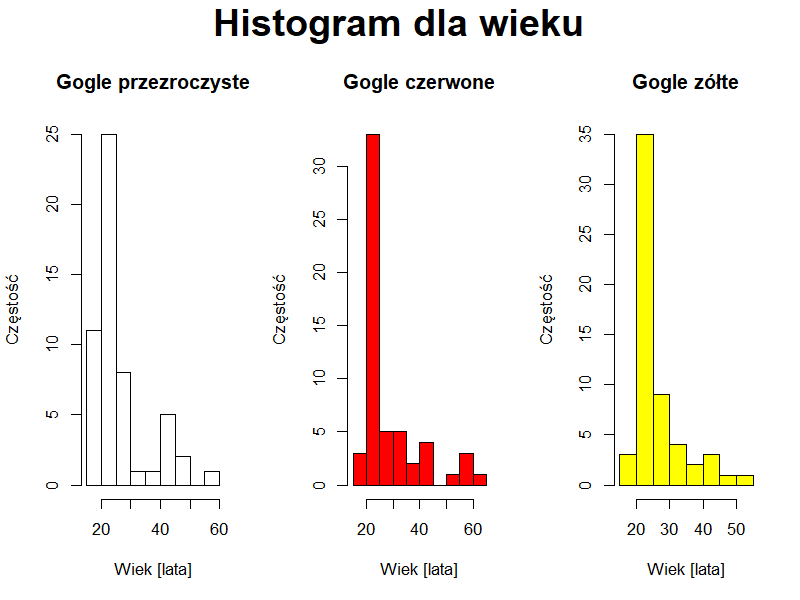
\includegraphics{./../res_plots/Histogram_dla_wieku.png}%
            }
            \label{fig:histAge}
        \end{figure}

        \begin{figure}[H]
            \centering
            \caption{Wykres pudełkowy dla wieku uczestników badania.}
            \resizebox{0.7 \columnwidth}{!}{%
            \includegraphics{./../res_plots/Wykres_pudełkowy_dla_wieku.png}%
            }
            \label{fig:boxAge}
        \end{figure}

        \subsubsection*{Doświadczenie zawodowe}
        \begin{table}[H]
            \centering
            \caption{Opis deskryptywny doświadczenia zawodowego uczestników badania.}
            \begin{tabular}{|c|c|c|c|}%
                \hline
                \bfseries Miara & \bfseries Gogle przezroczyste & \bfseries Gogle czerwone & \bfseries Gogle żółte% specify table head
                \csvreader[head to column names]{./../res_tables/summaryExperience.csv}{}% use head of csv as column names
                {\\\hline\Miara & \num{\T} & \num{\R} & \num{\Y}}% specify your columns here
                \\\hline    
            \end{tabular}
            \label{tab:summaryExperience}
        \end{table}

        \begin{figure}[H]
            \centering
            \caption{Histogram dla doświadczenia zawodowego uczestników badania.}
            \resizebox{0.7 \columnwidth}{!}{%
            \includegraphics{./../res_plots/Histogram_dla_doświadczenia_zawodowego.png}%
            }
            \label{fig:histExperience}
        \end{figure}


        \subsubsection*{Wyniki testu \textit{''health and safety''} (H\&S)}
        \begin{table}[H]
            \centering
            \caption{Opis deskryptywny wyników testu \textit{''health and safety''} (H\&S) uczestników badania.}
            \begin{tabular}{|c|c|c|c|}%
                \hline
                \bfseries Miara & \bfseries Gogle przezroczyste & \bfseries Gogle czerwone & \bfseries Gogle żółte% specify table head
                \csvreader[head to column names]{./../res_tables/summaryHSTestResults.csv}{}% use head of csv as column names
                {\\\hline\Miara & \num{\T} & \num{\R} & \num{\Y}}% specify your columns here
                \\\hline    
            \end{tabular}
            \label{tab:summaryHSTestResults}
        \end{table}

        \begin{figure}[H]
            \centering
            \caption{Histogram dla wyników testu \textit{''health and safety''} (H\&S) uczestników badania.}
            \resizebox{0.7 \columnwidth}{!}{%
            \includegraphics{./../res_plots/Histogram_dla_wyników_testu_H&S.png}%
            }
            \label{fig:histHSTestResults}
        \end{figure}

        \begin{figure}[H]
            \centering
            \caption{Wykres pudełkowy dla wyników testu \textit{''health and safety''} (H\&S) uczestników badania.}
            \resizebox{0.7 \columnwidth}{!}{%
            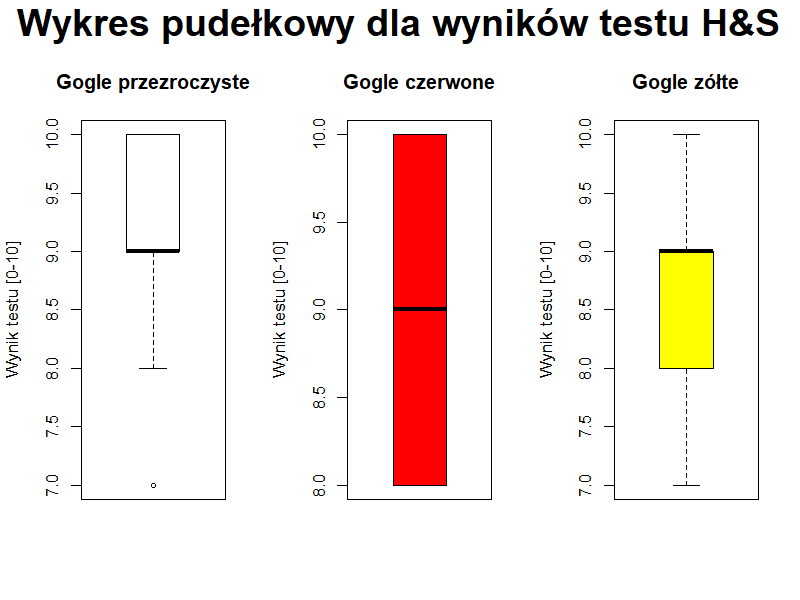
\includegraphics{./../res_plots/Wykres_pudełkowy_dla_wyników_testu_H&S.png}%
            }
            \label{fig:boxHSTestResults}
        \end{figure}

        \subsubsection*{Płeć}
        \begin{table}[H]
            \centering
            \caption{Opis deskryptywny płci uczestników badania.}
            \begin{tabular}{|c|c|c|c|}%
                \hline
                \bfseries Miara & \bfseries Gogle przezroczyste & \bfseries Gogle czerwone & \bfseries Gogle żółte% specify table head
                \csvreader[head to column names]{./../res_tables/summarySex.csv}{}% use head of csv as column names
                {\\\hline\Miara & \num{\T} & \num{\R} & \num{\Y}}% specify your columns here
                \\\hline    
            \end{tabular}
            \label{tab:summarySex}
        \end{table}

        \begin{figure}[H]
            \centering
            \caption{Histogram dla płci uczestników badania.}
            \resizebox{0.7 \columnwidth}{!}{%
            \includegraphics{./../res_plots/Histogram_dla_płci.png}%
            }
            \label{fig:histEsx}
        \end{figure}


    \subsection{Czas noszenia gogli}
    \begin{table}[H]
        \centering
        \caption{Opis deskryptywny czasu noszenia gogli uczestników badania.}
        \begin{tabular}{|c|c|c|c|}%
            \hline
            \bfseries Miara & \bfseries Gogle przezroczyste & \bfseries Gogle czerwone & \bfseries Gogle żółte% specify table head
            \csvreader[head to column names]{./../res_tables/summaryTime.csv}{}% use head of csv as column names
            {\\\hline\Miara & \num{\T} & \num{\R} & \num{\Y}}% specify your columns here
            \\\hline    
        \end{tabular}
        \label{tab:summaryTime}
    \end{table}

    \begin{figure}[H]
        \centering
        \caption{Histogram dla czasu noszenia gogli uczestników badania.}
        \resizebox{0.7 \columnwidth}{!}{%
        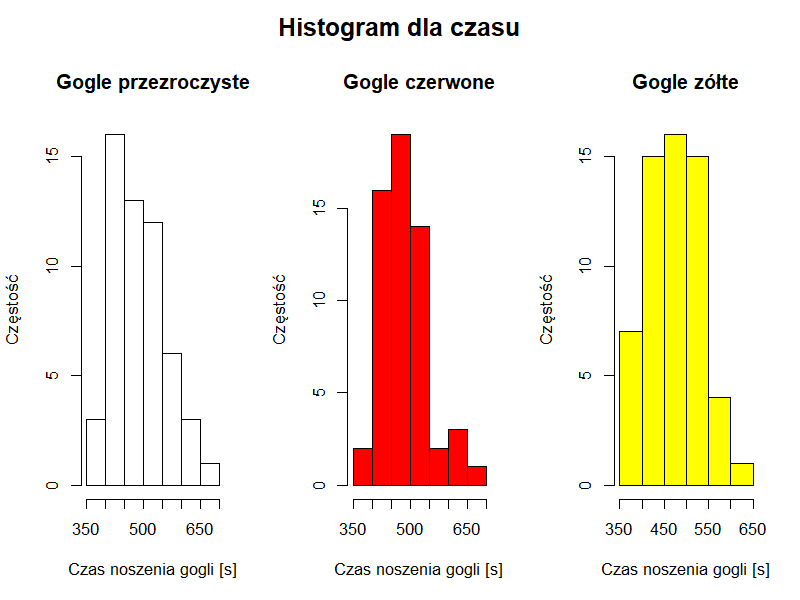
\includegraphics{./../res_plots/Histogram_dla_czasu.png}%
        }
        \label{fig:histTime}
    \end{figure}

    \begin{figure}[H]
        \centering
        \caption{Wykres pudełkowy dla czasu noszenia gogli uczestników badania.}
        \resizebox{0.7 \columnwidth}{!}{%
        \includegraphics{./../res_plots/Wykres_pudełkowy_dla_czasu.png}%
        }
        \label{fig:boxTime}
    \end{figure}